\newpage
\hypertarget{static:starting vis}{}
\subsection{Getting started in EA}
\visHeader
  
{\bf Note:} To continue with Part I's Demo files, open the \texttt{demo.eap} file in EA and ignore the first instruction below.

\begin{itemize}

\item[$\blacktriangleright$]  To begin, navigate to ``New Metamodel Project,'' and start a new visual project (this time without the demo specifications)
named \texttt{Leit\-ners\-Learn\-ing\-Box} (Fig.~\ref{fig:new_visModel}). Open the empty \texttt{.eap} file in EA.

\vspace{0.5cm}

\begin{figure}[htbp]
	\centering
  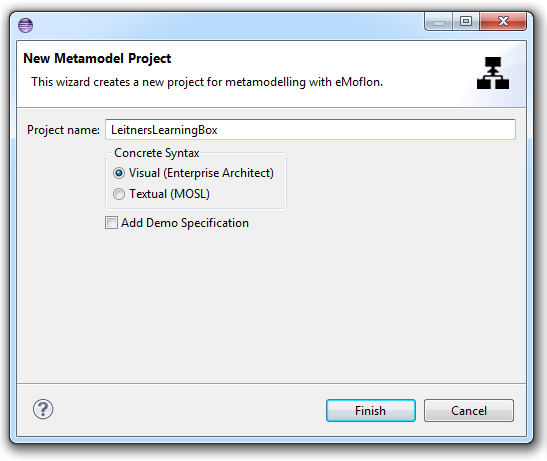
\includegraphics[width=0.8\textwidth]{eclipse_visNewMetamodelPlain}
	\caption{Starting a new visual project}
	\label{fig:new_visModel}
\end{figure}

\vspace{0.5cm}

\item[$\blacktriangleright$] In EA, select your working set and press the ``Add a Package'' button (Fig.~\ref{fig:new_package}). 

\begin{figure}[htbp]
	\centering
  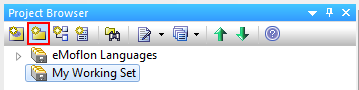
\includegraphics[width=0.5\textwidth]{ea_addPackage}
	\caption{Add a new package to \texttt{MyWorkingSet}}
	\label{fig:new_package}
	\vspace{0.5cm}
\end{figure}

\clearpage

\item[$\blacktriangleright$] In the dialogue that pops up (Fig.~\ref{fig:new_package_name}), enter \texttt{LearningBoxLanguage} as the name of the new
package. Make sure \texttt{Class View} is selected, and click \texttt{OK}.

\vspace{0.5cm}

\begin{figure}[htbp]
	\centering
    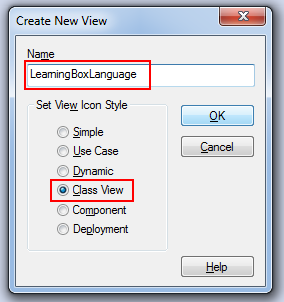
\includegraphics[width=0.33\textwidth]{ea_nameEPackage.png}
	\caption{Enter the name of the new package}
	\label{fig:new_package_name}
\end{figure}
\FloatBarrier

\vspace{0.5cm}

\item[$\blacktriangleright$] Your \texttt{Project Browser} should now resemble Fig.~\ref{fig:new_package_completed}.

\vspace{0.5cm}

\begin{figure}[htbp]
	\centering
  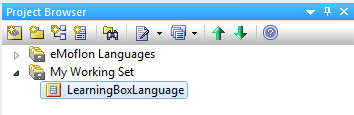
\includegraphics[width=0.5\textwidth]{ea_newPackage}
	\caption{State after creating the new package.}
	\label{fig:new_package_completed}
\end{figure}
\FloatBarrier


\vspace{0.5cm}

\item[$\blacktriangleright$] Now select your new package and create a ``New Diagram'' (Fig.~\ref{fig:diagram}).

\vspace{0.5cm}

\begin{figure}[htbp]
	\centering
  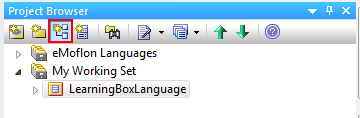
\includegraphics[width=0.5\textwidth]{ea_addDiagram}
	\caption{Add a diagram.}
	\label{fig:diagram}
\end{figure}
\FloatBarrier

\clearpage

\item[$\blacktriangleright$] In the dialogue that appears (Fig.~\ref{fig:diagram_type}), choose \texttt{eMoflon Ecore Diagrams} and press \texttt{OK}. 

\begin{figure}[htbp]
	\centering
  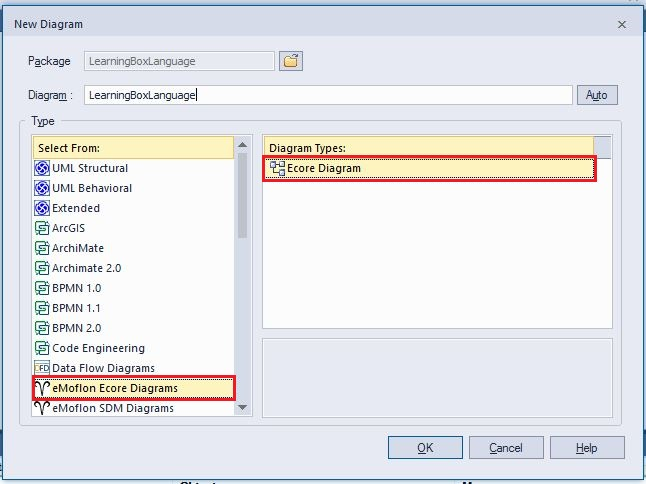
\includegraphics[width=0.8\textwidth]{ea_chooseDiagramType}
	\caption{Select the ecore diagram type}
	\label{fig:diagram_type}
\end{figure}
\FloatBarrier

 
\item[$\blacktriangleright$] After creating the new diagram, your  \texttt{Project Browser} should now resemble Fig.~\ref{fig:diagram_completed}. You'll notice
that your \texttt{LearningBoxLanguage} package has been transformed into an EPackage.

\begin{figure}[htbp]
	\centering
  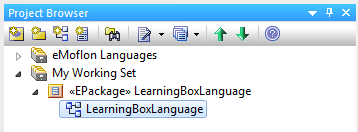
\includegraphics[width=0.5\textwidth]{ea_afterDiagramState}
	\caption{State after creating diagram}
	\label{fig:diagram_completed}
\end{figure}
\FloatBarrier

\item[$\blacktriangleright$] You can now already export your project to Eclipse,\footnote{If unsure how to perform this step, please refer to Part I, section
2.1} then refresh your \texttt{Package Explorer}. A new node, \texttt{My Working Set}\footnote{If you do not have the two distinct nodes, ensure your ``Top
Level Elements'' are set to \texttt{Working Sets}} should have appeared containing your EPackage (Fig.~\ref{fig:init_export}). You can see that a
\texttt{LearningBoxLanguage.ecore} file has been generated, and placed in ``model.'' This is your metamodel that will contain all future types you create in
your diagrams.

\clearpage

\vspace*{2cm}

\begin{figure}[htbp]
	\centering
  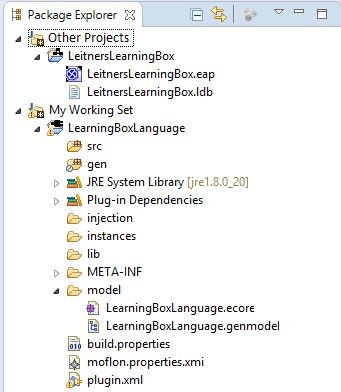
\includegraphics[width=0.55\textwidth]{eclipse_visInitExport}
	\caption{Inital export to Eclipse}
	\label{fig:init_export}
\end{figure}

\vspace{1cm}

\item[$\blacktriangleright$] If you're interested in reviewing the overall project structure, the purposes of certain files and folders, read section 4.1 from
Part~I. Otherwise, continue to the next to section learn how to declare classes and attributes.

\fancyfoot[R]{$\triangleright$ \hyperlink{static:classes vis}{Next}}
\end{itemize}
